\chapter{A technique to estimate defect probabilities} \label{chap:methods}

\section*{}
In this chapter it is discussed the methodologies used to validate the research questions.

\section{Schwa}
Schwa is the tool developed for research. Source code is available at Github\footnote{\url{https://github.com/andrefreitas/schwa}} as an Open Source project under MIT 2.0 license. It was developed in Python and is hosted at PyPi\footnote{\url{https://pypi.python.org/pypi/Schwa}}, the Python Package Index. 

\subsection{Installation}
Schwa relies on Python 3 and Git and they are the only dependencies. Can be easily installed using pip \footnote{\url{https://pip.pypa.io/en/latest/installing.html}}. 

\begin{lstlisting}[language=bash, caption=Schwa installation command]
   pip3 install schwa --pre
\end{lstlisting}

\subsection{Usage}
It can be used as a command line tool and imported as a Python package.

\begin{lstlisting}[language=bash, caption=Schwa CLI options]
usage: schwa [-h] [--commits COMMITS] repository

Predicts defects from GIT repositories.

positional arguments:
  repository         repository full path on local file system

optional arguments:
  -h, --help         show this help message and exit
  --commits COMMITS  maximum number of commits, since the last one, to be
                     analyzed
\end{lstlisting}

An example of running Schwa, is analyzing the last 20 commits of the Joda Time repository:

\begin{lstlisting}[language=bash, caption=Running Schwa on Joda Time]
schwa git/joda-time --commits 20
\end{lstlisting}

\subsection{Visualization}

\begin{figure}[H]
    \begin{center}
        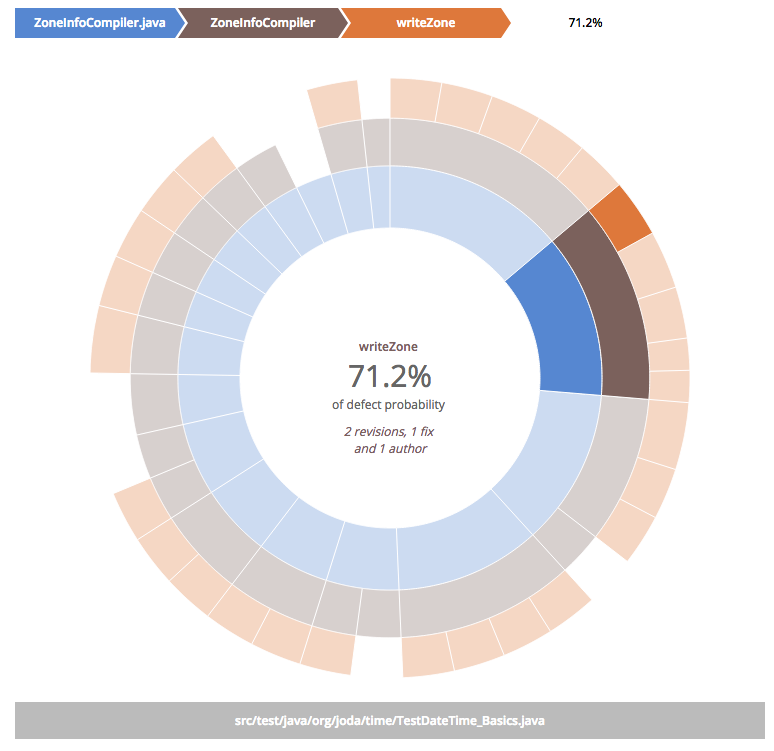
\includegraphics[scale=0.5]{schwa-sunburst}
        \caption{Sunburst results for Joda Time}
        \label{figure:sunburst-joda}
    \end{center}
\end{figure}

The report is launched in a browser and is displayed in a Sunburst chart, that is a simple way of showing an hierarchy of results. It is inspired from the visualization style of Crowbar. Granularity of components increases from the center to the periphery and the longer the arc, the higher the probability of defect. Blue nodes are files, brown are classes and orange are methods. The path of selected files are displayed in the bottom.

This visualization also gives some reasoning about the defect probability, displaying the values for revisions, fixes and authors.

\subsection{Process}
Mining a Software repository can be essentially divided in two phases: Extraction and Analysis. The rationale is that first we only extract the most important information and then extracted data is analyzed. By using a generic representation of a repository as the input for the analysis, Schwa can be extended with more SCM tools, such as Mercurial and Apache Subversion, due the modularity of this approach.


\begin{figure}[H]
    \begin{center}
        
\includegraphics[scale=0.5]{process}
        \caption{Process pipeline}
        \label{figure:schwa_process}
    \end{center}
\end{figure}

\subsubsection{Extraction}
Extraction is the phase that takes more time due the amount of I/O operations reading blobs, even with code parallelization. Considering these performance issues, Schwa iterates over commits, so it is possible to just extract for example, the last 10 commits, that most of the times is enough, considering that bugs have been introduced in the most recent changes. For each commit every change is parsed so the most important information is:

\begin{itemize}
\item  \textbf{Message} Commit message that is used to evaluate if the commit is fixing a bug;
\item  \textbf{Author} Commit author's email to track the number of contributors a component had;
\item  \textbf{Timestamp} An integer with the Unix Timestamp, used to track changes in components and achieving time relevance (TWR), that is distinguishing recently changed components from old components;
\item  \textbf{Diffs} The list of commit changes in components, such as files, classes and methods.
\end{itemize}

Schwa extracts data from Git repositories using the GitPython library\footnote{\url{https://github.com/gitpython-developers/GitPython}}. We achieved method granularity for Java source files and for other languages the granularity is at the file level. Parsing Java is possible by using the Plyj \footnote{\url{https://github.com/musiKk/plyj}} library, that has been modified to include line information for Classes and Methods in the Abstract Syntax Tree.

When the extraction finishes, all the important information has been collected and is represented in the model of figure \ref{figure:repository_model}. Note that this model is a balance of achieving performance and modularity.

\begin{figure}[H]
    \begin{center}
        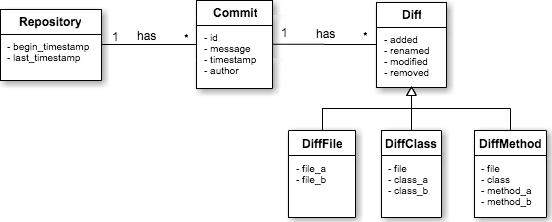
\includegraphics[scale=0.6]{Repository}
        \caption{Repository Model}
        \label{figure:repository_model}
    \end{center}
\end{figure}

Begin and last timestamps in the Repository class are referring to the first and last commits and are necessary for the TWR formula. Diffs have been divided in subclasses for each granularity. A diff is a result of changing a version A resulting in another version B. To make more clear this concept, consider the following patch:

\begin{lstlisting}[language=java, caption=Patch in API.java]
class API {
  static void login(String email, String password,
  AsyncHttpResponseHandler responseHandler){
      RequestParams params = new RequestParams();
      params.put("email", email);
      params.put("password", password);
+     params.put("token", "j76g367f4");
      client.post(url + "/login", params, responseHandler);
  }
  
+  static void getShows(AsyncHttpResponseHandler responseHandler) {
+   client.get(url + "/shows", responseHandler);
+  }

-  static void getUsers(AsyncHttpResponseHandler responseHandler) {
-   client.get(url + "/users", responseHandler);
-  }
}
\end{lstlisting}


The list of diffs instances would be:

\begin{lstlisting}[language=python, caption=List of Diff instances]
DiffFile(file_a="API.java", file_b="API.java", modified=True)
DiffClass(file_name="API.java", class_a="API", class_b="API", modified=True)
DiffMethod("API.java", class_name="API", method_a="login", method_b="login", modified=True)
DiffMethod("API.java", class_name="API", method_b="getShows", added=True)
DiffMethod("API.java", class_name="API", method_a="getUsers", removed=True)
\end{lstlisting}


To prove the flexibility of this model of representing diffs, if API.java would be renamed to RestAPI.java and therefore the class, the diffs would be:

\begin{lstlisting}[language=python, caption=Diff instances for a renamed class]
DiffFile(file_a="API.java", file_b="RestAPI.java", modified=True)
DiffClass(file_name="RestAPI.java", class_a="API", class_b="RestAPI",
renamed=True)
\end{lstlisting}

But, we are currently supporting only renaming of files since detecting a renaming of a Class or Method can be subjective. For example, it is not trivial by parsing a patch, recognizing the difference of deleting and creating a new method with the same body or only changing the method signature.

\subsubsection{Analysis}
Analysis receives a Repository as the input and will iterate again over commits but now with the objective of tracking the following metrics: 

\begin{itemize}
\item \textbf{Revisions} The more a component had recently new changes, the higher will be revisions score. Graves \textit{et al.} showed that revisions is a predictive variable \cite{859533};
\item \textbf{Fixes} The more a component had recently new bug-fixes, the higher will be fixes score; Zimmerman \textit{et al.} showed that past defects has the highest correlation with future defects \cite{Zimmermann:2007:PDE:1268984.1269057};
\item \textbf{Authors} The more a component had recently new authors, the higher will be authors score. Authors is a process metric that can be also used to predict defects \cite{Moser:2008:CAE:1368088.1368114,D'Ambros:2012:EDP:2318097.2318149}.
\end{itemize}

Metrics are tracked the same way for any granularity and they were selected after a revision of the state of the art in MSR. 
Considering our goal of improving Crowbar fault localization results, the Time-Weighted Risk approach is the one that fits this scenario, since it is a rank-based technique. TWR is not only used only for Fixes but also for Revisions and Authors, since they can benefit of time relevance, something that was not possible when using counters.

We also found that the TWR curve in the Figure \ref{figure:twr_graph}, should be modified, because even recently changed components were having low score. The problem, is that when \( t_i <= 0.8 \), TWR is low. We want the curve to start growing sooner so therefore we modified the TWR equation with the Time Range (TR) parameter, resulting in a new expression:

\begin{equation}
twr(t_i) = \frac{1}{1 + e^{-12t_i + 2 + ( (1 - TR)* 10) }}
\end{equation}

TR varies from 0 to 1 and the more we increase it, the curve goes to the left as visible in \ref{figure:twr_modified_graph}.

\begin{figure}[!ht]
    \begin{center}
        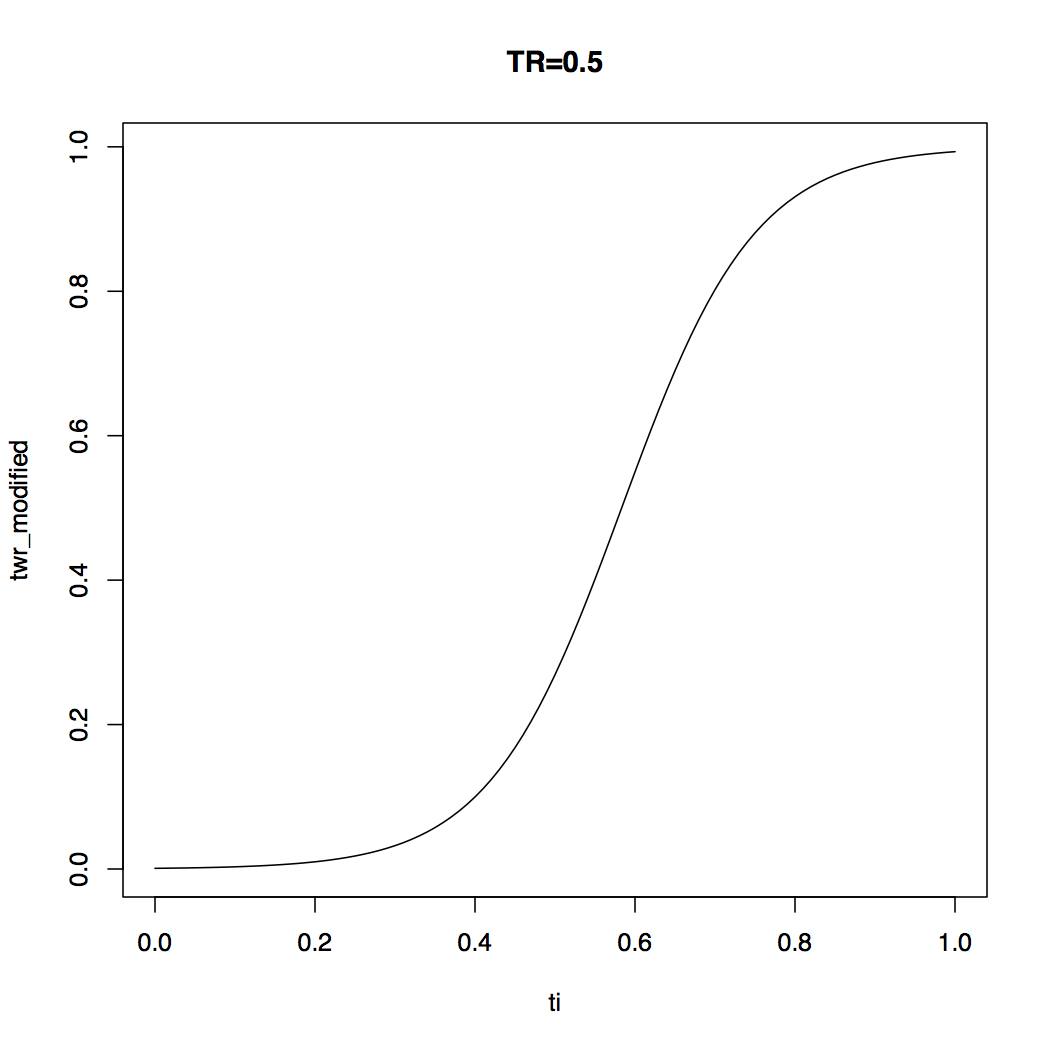
\includegraphics[scale=0.5]{twr_modified_graph}
        \caption{Modified Time Weighted Risk (TWR)}
        \label{figure:twr_modified_graph}
    \end{center}
\end{figure}

With a deeper understanding about how TWR works, algorithm \ref{algorithm:analysis} describes the steps involved in the analysis, in a simplified way.\*

\begin{algorithm}[H]
\For{each commit in the repository}{
  twr = compute twr
  
  \For{each component in the commit}{
    component.revisions += twr
    
    \If{commit is bug fix}{
        component.fixes += twr
    }
    
    \If{is new author}{
        component.authors += twr
    }
  }
}
\caption{Analysis algorithm}
\label{algorithm:analysis}
\end{algorithm}

We detect if a commit is fixing a bug by searching for keywords in the message. Since Github\footnote{\url{http://github.com}} is the most used Git repository hosting service, the regular expression was based on Github's syntax for closing issues by commit messages \footnote{\url{https://help.github.com/articles/closing-issues-via-commit-messages/}}. The regular expression is the following:

\begin{lstlisting}[language=python, caption=Bug-fixing message regular expression]
fix(e[ds])?|bugs?|defects?|patch|close([sd])?|resolve([sd])?
\end{lstlisting}

\subsubsection{Defect prediction computation}
When the analysis is finished, Schwa computes the defect probability for every component by doing a weighted average of the metrics: 

\begin{equation}
score = revisions * revisions_{weight} + fixes * fixes_{weight} + authors * authors_{weight}
\end{equation}

Then the score is normalized to a value from 0 to 1, that is the estimation of the defect probability:

\begin{equation}
defect_{probability} = 1 - e^{-score}
\end{equation}

By default, Schwa uses the weights: 0.25 for revisions, 0.25 for authors and 0.5 for fixes. These weights are based from literature and observation \cite{859533, Zimmermann:2007:PDE:1268984.1269057, Moser:2008:CAE:1368088.1368114,D'Ambros:2012:EDP:2318097.2318149}. They may be different for each type of software project. For example, in a project with a lot of contributors, tracking authors can be important, but in a project with just a contributor, this metric is not relevant.

\section{Features weight estimation}
Estimating the weights of each feature: revisions, fixes and authors is an optimization problem. Our approach was using Genetic Algorithms for searching the best solution and encoding individuals as:

\begin{equation}
\{R, F, A\}
\end{equation}

$R$, $F$ and $A$ are the weights from 0 to 1 for revisions, fixes and authors, respectively. They have been encoded to binary with 3 bits of precision, that means that we can represent \( 2 ^3 = 9 \) different values for each feature. Increasing bits precision has the cost of decreasing performance. 

The fitness function \ref{eq:fitness_ga} is the sum of the distance between involved and not involved components for every bug-fixing commit \(m\) with a penalty for invalid solutions: weights cannot be 0 and their sum must be 1. This rationale results in the following expressions:

\begin{equation}
\label{eq:fitness_ga}
fitness(R,F,A) =
  \begin{cases} 
      \hfill \sum_{m \in commits_{bugfixing}}^{} distance(R,F,A,m)  \hfill & \text{ if constraints($R$,$F$,$A$)}\\
      \hfill -\infty \hfill & \text{ else} \\
  \end{cases}
\end{equation}

\begin{equation}
constraints(R,F,A) = (R+F+A) = 1 \wedge (R*F*A) > 0
\end{equation}

\begin{equation}
distance(R,F,A,m) = \frac{ \sum_{c \in involved(m)}^{} score(R,F,A,c) }{|involved(m)|} - \frac{ \sum_{c \in (Components \setminus involved(m))}^{} score(R,F,A,c) }{|(Components \setminus involved(m))|}
\end{equation}

\begin{equation}
score(R,F,A,c) = c_{revisions} * R + c_{fixes} * F + c_{authors} * A
\end{equation}

This means that in bug-introducing commits, faulty components should have higher score than non faulty components. Besides finding features weights, this approach help us validate if Schwa is predicting defects correctly. Due performance constraints, the fitness function only evaluates components at the file granularity.

\section{Diagnostic cost}
Crowbar outputs a rank of components ordered by their probability of having the fault. To measure the quality of this diagnostic, the heuristic used is Diagnostic Cost \cite{6693085} that is the average of the minimum and maximum distance that faulty components are from the top of the rank. For multiple faults, this cost is computed considering the lowest faulty component.

\begin{equation}
diagnostic_{cost} = \frac{min_{distance} + max_{distance} - |faulty|}{2}
\end{equation}

\subsection{Example}
\( C_2 \) is the component that have the fault.

\begin{table}[h]
\centering
\caption{Examples of ranks}
\label{my-label}
\begin{tabular}{|c|c|c|}
\hline
Position & Rank 1 & Rank 2 \\ \hline
    1    &   \( C_3(0.234) \)   &  \( *C_2(0.500) \)     \\ \hline
    2    &   \( C_5(0.145) \)   &  \( C_5(0.120) \)     \\ \hline
    3    &   \( *C_2(0.145) \)   &  \( C_3(0.120) \)   \\ \hline
    Diagnostic Cost   &   1   &  0  \\ \hline
\end{tabular}
\end{table}

In Rank 1 \(C_5\) and \(C_2\) components have the same probability so \(C_2\) position can be 2 or 3 depending on the result of ordering the rank. In Rank 2 \(C_2\)  is on the first position so the cost is 0.

\subsection{Schwa integration with crowbar}
By using Schwa, the goal is improving Barinel results, reducing the Diagnostic Cost by evaluating if defect probabilities should be used in priors ($p_j$), goodness ($g_j$) or both parameters. 

\begin{description}
\item[Prior] \hfill \\
The probability a component have of causing an error and is by default \( \frac{1}{1000} \), based on the heuristic that for every 1000 lines of code heuristic there is one bug. 
\item[Goodness] \hfill \\
The probability of a component behaving normally and by default is computed by using the Maximum Likelihood Estimation that is heavy to compute. By default is $0.5$.
\end{description}

If the defect probability of Schwa is used for goodness, it is computed by:
\begin{equation}
\pr(obs_i,e_i \mid d) = 1 - defect_{probability}(c)
\end{equation}
